\documentclass[12pt]{article}

\usepackage{EngReport}
\usepackage{titleref}
\makeatletter
\newcommand*{\currentname}{\TR@currentTitle}
\makeatother

\graphicspath{{Images/}}
\bibliography{Sources}
\onehalfspacing
\graphicspath{{images/}}
\geometry{letterpaper, portrait, includeheadfoot=true, hmargin=1in, vmargin=1in}

%\fontsize{font size}{vertsize (usually 1.2x)}\selectfont

\begin{document}
\renewcommand{\familydefault}{\rmdefault}

\begin{titlepage}
    \begin{center}
    {\fontsize{36}{42}\selectfont \bfseries Exploring Camunda} 
    \\\vspace{20pt}
    {\LARGE Journey to learning Camunda} \\
    \vspace{20pt}
    \textbf{Amine Neggazi}
    \vspace{8pt}
    \\Prepared for, 23 / 07 / 2023
    \end{center}
\end{titlepage}

\pagestyle{fancy}
\fancyhf{}
\setlength{\headheight}{30pt}
\renewcommand{\headrulewidth}{0.4pt}
\renewcommand{\footrulewidth}{0.4pt}
\lhead{\large ** Section ** }
\rhead{\large ** Subsection ** }
\rfoot{\textbf{Page \thepage}}
\lfoot{}

\tableofcontents

\fontsize{12}{20}\selectfont{

\pagebreak

\section{Introduction}

In this article, I will share my journey of learning Camunda, an open-source platform for workflow and decision automation. As businesses strive for efficiency and agility, understanding tools like Camunda becomes crucial for streamlining processes and optimizing operations. I am very motivated to explore this powerful platform, and I embarked on a learning adventure to uncover the possibilities it offers.

Throughout this article, I will provide insights into the fundamentals of BPMN (Business Process Model and Notation) and its role in visualizing and modeling business processes. I will then dive into my experience with Camunda after using it in a small project, I'll also give a brief step by step learning journey from the initial installation and setup to exploring the Camunda Modeler, which allowed me to create clear and concise process diagrams.

I will also share valuable lessons learned,

  \subsection{Motivation and Goals}

I am motivated to learn camunda as it is a necessary tool for infrastructure automation and to also enhance productivity.
Here are some goals that I want to accomplish:

\begin{itemize}
  \item Gain a solid understanding of BPMN.
  \item Understand camunda's workflow engine.
  \item Effectively model and automate complex business processes.
  \item Camunda integration with other systems.
  \item Collaboration with co-workers.
\end{itemize}

\pagebreak

\section{What is BPMN ?}

  \subsection{Introduction}

Business Process Model and Notation was developed as a graphical notation to represent complex processes and address these challenges. It is maintained by the non-profit The Object Management Group (OMG) and employed by numerous organizations globally. The visual nature of BPMN enables greater collaboration between different teams.

  \subsection{Basics of BPMN}

Here are the foundational elements of BPMN:

  \begin{itemize}
    \item Process.
    \item Activities (Tasks, Sub-Processes, and Call activities).
    \item Events (Start Events, Intermediate Events, and End Events).
    \item Gateways (Exclusive, Parallel, and Inclusive Gateways)
    \item Sequence Flow.
    \item Data Objects.
  \end{itemize}

\pagebreak

Here is a figure representing BPMN components:

\begin{figure}[h]
    \centering
    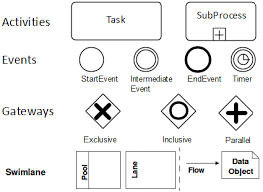
\includegraphics[width=.35\linewidth]{bpmn.png}
    \caption{BPMN components}
    \label{fig:bpmn}
\end{figure}

  \subsection{Learning Process and Resources}
I started by learning the concepts of each elements used in BPMNs (tasks, symbols, activities...), and then since I had previous knowledge of modeling languages and UML diagrams, so it all seemed similiar.
Then, I created some simple examples :
\\
One of them was automating a Car Starting System (Each car executes some checks before starting).
I also read some best practices on using BPMNs.

\section{What is Camunda ?}

  \subsection{Introduction}

Camunda is an open-source platform for workflow and decision automation. It provides a powerful workflow engine, BPMN modeling capabilities, and tools for managing and executing business processes. With Camunda, organizations can automate and optimize their business processes, improve efficiency, and enhance visibility into process execution.

\pagebreak

  \subsection{Installation and Setup}

Camunda is fairly simple to install (for me I installed it in linux):

  \begin{itemize}
    \item Downloading Camunda Platform 7 Community edition from (https://camunda.com/download/) the linux version comes in Zip and Tar formats.
    \item Extract the Zip / Tar.
    \item Run the script `./start.sh` to launch camunda platform.
    \item Now we can navigate to `http://localhost:8080/camunda-welcome/index.html` and explore camunda features.
  \end{itemize}

\pagebreak

\section{Creating a Simple Process}

  \subsection{Designing a Process}
  
For this section, I have decided to implement a small simple project using BPMN in Camunda to learn more about it.
For designing the process, here are the steps I did to implement a new employee integration system:

\begin{itemize}
  \item A start process is initiated to start the process of employee integration.
  \item A first task (user task) is created that represents collecting user information such as Identification, employment forms, certifications..etc
  \item The next task is assigning the new employee to various tasks and departements.
  \item Next, we execute parralel tasks (first one is a user task which orients the new employee and provides information about company policies, culture, and team introductions, and the second task is a service task which is used to automate generating welcome emails, provisioning accounts, and preparing employee workstations).
  \item The last task is reviewing all the documents by the HR departement to confirm completion of all tasks.
  \item and now the end event is triggered to end the process.
\end{itemize}

\pagebreak

Here is how the implemented simple process looks like:

\begin{figure}[h]
    \centering
    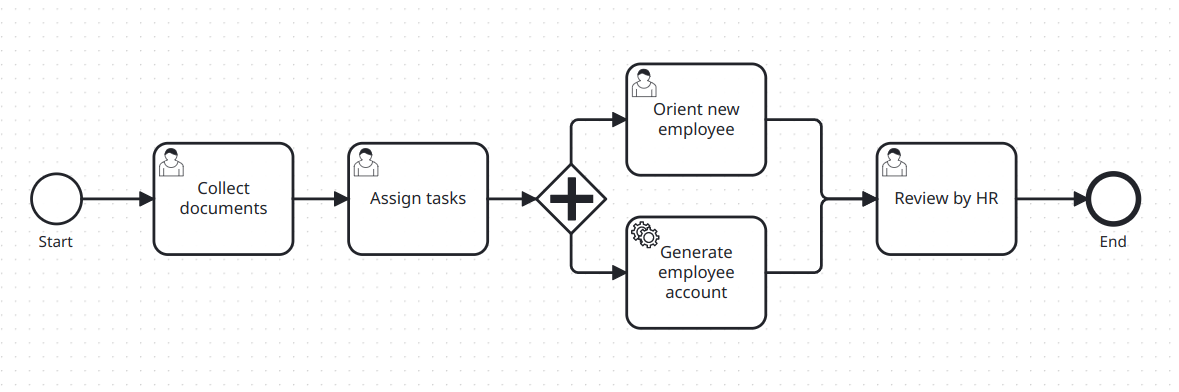
\includegraphics[width=.90\linewidth]{simple_process.png}
    \caption{Simple Process}
    \label{fig:simple_process}
\end{figure}

  \subsection{Executing the Process}

Here is the process I used to deploy and execute the process:

\begin{itemize}
  \item First, I exported the BPMN file which contains the XML representation.
  \item Then, we can access it on `http://localhost:8080/camunda/app/cockpit` by loggin in using demo / demo as a username and password.
  \item We now can create a deployment by importing the BPMN file.
  \item We then check for the state of the process.
  \item Now, we can go to the tasklist which is accessible on `http://localhost:8080/camunda/app/tasklist` and start the process.
  \item Finally by checking on Camunda Cockpit, we can see that there is an instance running on the first task.
\end{itemize}

  \subsection{Adding an external task (service task)}

In this section I will be implementing small script in python that will be integrated with camunda as a service task.

Here are the steps it took me to implement it (following instructions from https://github.com/camunda-community-hub/camunda-external-task-client-python3):

\begin{itemize}
  \item First I initialized a new python project using a python virtual environment `python -m venv venv`, then sourcing the `venv/bin/activate` script to activate the python virtual environment.
  \item Next, I installed the camunda external task client using the command `pip install camunda-external-task-client-python3`
  \item Then, I used the command `pip freeze $ > $ requirements.txt` to save all the dependencies.
  \item I then created a simple BPMN process using camunda modeler which contains a service task which has a topicName (for integration) as you can see in figure \ref{fig:service_task}.
  \item Then, I deploy that process locally `http://localhost:8080/camunda/app/cockpit`.
  \item Next, I added the python code from camunda python external client repo (https://github.com/camunda-community-hub/camunda-external-task-client-python3)
\end{itemize}

\begin{figure}[h]
    \centering
    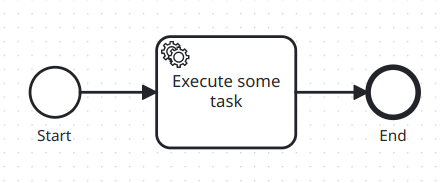
\includegraphics[width=.50\linewidth]{service_task.png}
    \caption{Service Task}
    \label{fig:service_task}
\end{figure}

\pagebreak

\section{What I Learned}

Here are some key points that I learned from using camunda:

\begin{itemize}
  \item Camunda as a whole and its benefits.
  \item The different components of the Camunda Platform.
  \item The basics of BPMN, the standard for process modeling.
  \item Creating processes using camunda modeler.
  \item Deploying and running process models using Camunda Platform.
\end{itemize}

\pagebreak

\section{Conclusion}

}

\printbibliography

\end{document}
